\documentclass[12pt,fleqn]{article}
\renewcommand{\baselinestretch}{1.3}
\usepackage{appendix,hyperref,harvard,amsmath,amssymb,lscape,graphicx,setspace,cancel,amsthm,pgfplots,fullpage}
\usepackage[nomarkers,notablist,nofiglist,fighead,tabhead]{endfloat}
%\usepackage{amsfonts,latexsym,eurosym}
\bibliographystyle{aer}

%\pdfpagewidth 8.5in
%\pdfpageheight 11in
%\topmargin 0in
%\headheight 0in
%\headsep 0in
%\textheight 9in
%\textwidth 6.5in
%\oddsidemargin 0in
%\evensidemargin 0in
%\headheight 0in
%\headsep 0in

\newcommand{\D}{\displaystyle}
\newcommand{\E}{\begin{eqnarray*}}
\newcommand{\F}{\end{eqnarray*}}
\newcommand{\EE}{\begin{eqnarray}}
\newcommand{\FF}{\end{eqnarray}}
\newcommand{\IZ}{\begin{itemize}}
\newcommand{\ZI}{\end{itemize}}
\newcommand{\EN}{\begin{enumerate}}
\newcommand{\NE}{\end{enumerate}}
\newcommand{\itemc}{\item[$\circ$]}
\newcommand{\IZdash}{\begin{itemize} \renewcommand{\labelitemi}{-}}
\newcommand{\tn}{\textnormal}

%\doublespacing
%\onehalfspacing

\pgfplotsset{height =7cm,compat=1.7,width=7cm,
    standard/.style={
    	unit vector ratio*=1 1 1,
        axis x line=middle,
        axis y line=middle,
        enlarge x limits=0.15,
        enlarge y limits=0.15,
        every axis x label/.style={at={(current axis.right of origin)},anchor=north west},
        every axis y label/.style={at={(current axis.above origin)},anchor=north east}
    }
}
\newcommand{\drawge}{-- (rel axis cs:1,0) -- (rel axis cs:1,1) -- (rel axis cs:0,1) \closedcycle}
\newcommand{\drawle}{-- (rel axis cs:1,1) -- (rel axis cs:1,0) -- (rel axis cs:0,0) \closedcycle}

\usetikzlibrary{patterns}
\usetikzlibrary{arrows}

%%%%%%%%%%%%%%%%%%%%%%%%%%%%%%%%%%%%%%%%%%%%%%%%%%%%%%%%%%%%%%%%%%%%%%%%%%%%%%%%%%%%%%%%%%%%%%%%%%%%
%%%%%%%%%%%%%%%%%%%%%%%%%%%%%%%%%%%%%%%%%%%%%%%%%%%%%%%%%%%%%%%%%%%%%%%%%%%%%%%%%%%%%%%%%%%%%%%%%%%%%

\begin{document}

%\begin{titlepage}
\title{Notes on New-Keynesian Business Cycle Modeling}
\author{
%Econ 107: Asymmetric Information\\
Brian Jenkins\\  University of California, Irvine}
\date{\today}

\maketitle
%\begin{abstract}

%\end{abstract}
%\thispagestyle{empty}
%\end{titlepage}

\newpage
\tableofcontents

\cleardoublepage
% \phantomsection
\addcontentsline{toc}{section}{\listfigurename}
\listoffigures

\cleardoublepage
% \phantomsection
\addcontentsline{toc}{section}{\listtablename}
\listoftables

\newpage
\section{The Model Setup}

The model that we analyze in this chapter is representative of the \textbf{new-Keynesian} models that are currently used to analyze the business cycle and to study monetary policy. The model is \emph{Keynesian} because nominal prices are not flexible; they adjust gradually in response to an exogenous shock to the economy. The model is \emph{new} because it is built upon a solid microeconomic foundation. The predictions of the model arise as the result of optimal behavior on the part of households and firms. With a micro-founded model, we will be able to see how the behavior of the aggregate economy over the business cycle is similar to how an individual households and firms might also behave during the business cycle. Furthermore, we will be able to exactly how the way in which monetary policy is conducted influences the equilibrium relationships between inflation, output, and interest rates.

\subsection{The Demand for Goods.}


The demand for goods and services is assumed to have the following linear relationship:
	\EE
	y_t & = & E_t y_{t+1}  - \left( r_{t+1} - \bar{r}\right) + g_t. \label{eqn:DynIS}
	\FF
Here, $y_t\equiv \log Y_t$ denotes natural log of real output, $r_{t+1}$ is the real interest rate on funds saved from period $t$ to $t+1$, and $\bar{r} \equiv -\log \beta$ is the steady state \emph{natural rate of interest}. The expression $E_t y_{t+1}$ means the expected value of (log) output in period $t+1$ given information about the economy available as of period $t$. The variable $g_t$ denotes an exogenous shock to the demand for goods and services and has an unconditional expectation of zero. We call equation (\ref{eqn:DynIS}) a \textbf{dynamic IS relationship} because it is based on equilibrium in the market for goods and services.

The dynamic IS relationship is based on a standard Euler equation for a representative household and is therefore closely related to the Euler equations that we have encountered before. The representative household that we should have in mind is one that chooses how much to consume and save each period based on its current income, its income in the following period, and the market real interest rate. In equilibrium, saving does not take place on the aggregate level, and so the real interest rate always adjusts so that the household is just satisfied with its income in the current period relative to the future.

The shock to aggregate demand $g_t$ reflects any exogenous fluctuation in the demand for goods. A \emph{positive} realization of $g_t$ reflects a temporary increase in the demand for goods that could be due to a temporary increase in government purchases, some short-term exuberance in the financial markets, or a variety of other things. Similarly, a \emph{negative} realization of $g_t$ would reflect a temporary \emph{decrease} in the demand for goods; perhaps because of a sudden reduction in the demand for net exports or a collapse in asset prices.

\subsection{The Fisher Equation}

The \textbf{Fisher equation} links nominal and real interest rates:
	\EE
	i_{t} & = & r_{t} + E_t \pi_{t+1},  \label{eqn:DynFisher}
	\FF
where $i_{t}$ is the nominal interest rate on funds saved from period $t$ to $t+1$, $r_{t}$ is the ex ante real interest rate earned over the same period, and $E_t \pi_{t+1}$ means the expected value of inflation in period $t+1$ given information about the economy available as of period $t$. Equation (\ref{eqn:DynFisher}) arises because financial business is conducted in nominal terms but people care about real quantities. Therefore, the nominal interest rate is determined by the expected rate of inflation and the desired real interest rate.

\subsection{Monetary Policy}

We suppose that monetary policy is set according to the following \emph{rule}:
	\EE
	i_{t} & = & \bar{r} + \pi^T + \phi_{\pi}\big(\pi_t - \pi^T\big) + \phi_{y}\big(y_t - \bar{y}\big) + v_t,  \label{DynMonetary}
	\FF
where $\bar{y}$ is the (log) natural rate of output and $v_t$ is an exogenous shock to monetary policy. $\pi^T$ is the central bank's \emph{target} for inflation. $\phi_{\pi}$ is the amount that the central bank raises the nominal interest rate in response to a one unit increase in the rate of inflation. $\phi_{y}$ is the amount that the central bank raises the nominal interest rate in response to a one unit increase in output. The size of $\phi_{\pi}$ relative to $\phi_y$ indicates the weight that the central place attaches to inflation stabilization relative to output stabilization. For reasons that will be discussed in more detail later, stability of the model requires $\phi_{\pi}>1$ and $\phi_y\geqslant0$. That is, for the model to predict a stable equilibrium, the central bank must respond to a one percent increase inflation by an increase in the nominal interest rate that is greater than one percent.

It might be surprising that we have a specification for monetary policy that does not explicitly mention the supply of money. You can think of equation (\ref{DynMonetary}) as determining a target for the nominal interest rate. The central bank then manipulates the supply of money in order to meet its target. This way of thinking is similar to how the Federal Reserve conducts monetary policy in the United States. The FOMC announces a target for the nominal interest rate and then the Federal Reserve Bank of New York conduct open market operations on a daily basis to make sure that the federal funds rate is equal to the target set by the FOMC. Among other advantages, setting policy this way means that fluctuations in the demand for money will be fully accommodated by the Federal Reserve and will therefore have no effect on the rest of the economy.


\subsection{The Supply of Goods}

We suppose the following aggregate supply relation:
	\EE
	\pi_t -\pi^* & = & \beta \left( E_t\pi_{t+1} - \pi^*\right)  + \kappa (y_t -\bar{y})+ u_t, \label{eqn:DynAS}
	\FF
where $\pi_t$ is the inflation rate between periods $t-1$ and $t$, $\pi^*$ is the steady state rate of inflation, $\bar{y}$ is the (log) natural rate of output, and $u_t$ is an exogenous shock to the rate of inflation. The expression $E_t \pi_{t+1}$ means the expected value of inflation in period $t+1$ given information about the economy available as of period $t$.

We will call equation (\ref{eqn:DynAS}) the \textbf{dynamic AS relationship}. The dynamic AS relationship implies that current inflation is positively related to current output and to expected future inflation. The dynamic AS relationship is the result of four fundamental assumptions about the firms that produce goods.  First, goods and services are produced by \emph{monopolistic competitors}. Second, the demand for the goods of each firm is proportional to the demand for all goods. Third, firms face rising marginal costs of production. And finally, each firm incurs a \emph{menu cost} when it changes the price of its product.


Unlike firms in perfectly competitive markets, monopolistic competitors face downward-sloping demand curves for their products and so they have the ability to set the prices of their products. Because we assume that the demand for goods from each firm is proportional to the demand for all goods, then an increase in household income will increase the demand for goods produced by each firm. Since firms face rising marginal costs of production, they would want to raise the prices of their products in response to an increase in the overall demand for goods.

But firms also find it costly to adjust their price from one period to the next and the cost is increasing with magnitude of the price change. When the demand for goods rises, firms might find it optimal to raise the prices of their products by less than the amount that would be required to fully counter the rise in demand and so an increase in demand can produce an increase in production.

Equation (\ref{eqn:DynAS}) is also routinely called the \textbf{new-Keynesian Phillips curve}. Strictly speaking, a \textbf{Phillips curve} reflects the relationship between inflation and unemployment. By recognizing the negative relationship between output and unemployment, equation (\ref{eqn:DynAS}) can easily be rewritten in terms of inflation and unemployment. As we will see below, the model will imply that there is no long-run relationship between inflation and output and therefore no long-run relationship between inflation and unemployment.




\section{Long-Run Equilibrium: The Steady State}

In the steady state, all exogenous variables are equal to zero:
	\EE
	g_t = v_t = u_t = 0.
	\FF
and all of the endogenous variables are constant. Using an asterisk to denote the steady state magnitude of a variable, we can obtain the following steady state relationships:
	\EE
	y^* & = & \bar{y}\\
	\pi^* & = & \pi^T\\
	r^* & = & \bar{r}\\
	i^* & = & \bar{r} + \pi^T
	\FF
In the steady state, output equals the natural rate of output that is consistent with the economy being on a smooth long-run growth path. The steady state real interest rate equals the natural rate of interest. Recall that $\bar{r} \equiv - \log  \beta$ which means that the real rate of interest is determined by the rate at which households discount future utility. Other things equal, greater discounting -- i.e., a \emph{lower} value for $\beta$ -- will result in a lower steady state real interest rate.

Finally, we can see that the central bank's target rate of inflation determines the steady state rate of inflation and the nominal interest rate. It is worth appreciating that this model is a general equilibrium model and provides a complete theoretical account of the determination of the long-run rate of inflation. The central bank obtains its target for inflation in the long-run by committing itself to adjusting the nominal interest rate whenever inflation deviates from the target.
	
\section{Calibration}

In order to analyze the model numerically, we have to select values for the various parameters of the model. Selecting parameters for a model is called \emph{calibration}. While there are more rigorous methods available, we will keep it simple. Table \ref{table_calib} contains the calibrated parameter values that we will use for our analysis.

\begin{table}[h] \caption{\label{table_calib} Calibrated parameters for the dynamic AS-AD model.}

\

\begin{center}\begin{tabular}{|c|c|} \hline \textbf{Parameter} & \textbf{Value}\\\hline
{\rule[3mm]{0mm}{0mm}} $\bar{y}$   & 0 \\
                       $\beta$     & 0.995\\
                       $\kappa$    & 0.25\\
                       $\pi^T$     & 0.02/4   \\
                       $\phi_{\pi}$& 1.5 \\
                       $\phi_{y}$  & 0.5/4\\\hline
\end{tabular}\end{center}
\end{table}

We will set the natural rate of output to 1 so steady state log output $\bar{y}$ is 0. Doing so means that we can simply interpret $y_t$ as the log deviation of output from the natural rate or steady state.\footnote{Because: $y_t - \bar{y} = \log Y_t - \log \bar{Y} \approx (Y_T - \bar{Y})/\bar{Y}$. It is common to refer to $y_t - \bar{y}$ as the \emph{output gap}.} We will assume a value of $\beta$ of 0.995 and this implies an annualized steady state real rate of interest of 2\%. Assume that $\kappa$ is 0.25 which means that every 1\% increase in output above the natural rate will increase the rate of inflation by 0.25\% on a quarterly basis.
	
Consistent with the Federal Reserve's recent statements, we will assume that the central bank's target for inflation is 2\%. We will take the coefficient on inflation in the monetary policy rule $\phi_{\pi}$ to be 1.5 and we will set the coefficient on output $\phi_y$ to 0.5/4. This means that the central bank will only adjust the nominal interest rate in response to both changes in inflation and output, but with a greater priority given to inflation fluctuations.

Finally, we have to make some assumptions about how the exogenous shocks evolve. We'll assume that each is an AR(1) process:
	\EE
	g_{t+1} & = & \rho_g g_{t} + \epsilon^g_{t+1}\\
	u_{t+1} & = & \rho_u u_{t} + \epsilon^u_{t+1}\\
	v_{t+1} & = & \rho_v v_{t} + \epsilon^v_{t+1}.
	\FF
For the simulations below will assume that $\rho_g = \rho_u =\rho_v = 0.5$. The variables $\epsilon^g_t$, $\epsilon^u_t$, and $\epsilon^v_t$ are white noise processes.


\section{Short-Run Fluctuations}

Here we examine how the exogenous shocks to the model produce business cycles.

\subsection{Temporary Demand Shock}

First we will consider the effect of a persistent shock to the demand for goods. To do this, we need to solve the model so that the endogenous variables are written as functions of only the exogenous state variables. Usually, solving dynamic models with forward-looking expectations is hard and so a numerical method like that provided by the Python module \verb=linearsolve= is required. But in the case of the new-Keynesian model, the solution can be obtained with a bit of (tedious) algebra. The advantage of deriving the solution by hand is that the hand-derived solution makes it clear how the various model parameters affect the solution.


To derive the solution with respect to the demand shock, assume that the demand shock is the only shock in the model and write the equilibrium equations as:
	\EE
	y_t & = & E_t y_{t+1}  - \left( r_{t} - \bar{r}\right) + g_t\\
	\pi_t -\pi^T & = & \beta \left( E_t\pi_{t+1} - \pi^T\right)  + \kappa (y_t -\bar{y})\\
	i_{t} & = & r_{t} + E_t \pi_{t+1}\\
	i_{t} & = & \bar{r} + \pi^T + \phi_{\pi}\left(\pi_t - \pi^T\right) + \phi_y \left(y_t - \bar{y}\right)
	\FF
Now, use the Fisher equation and the monetary policy rule to eliminate the nominal interest rate and the real interest rate from the model:
	\EE
	y_t & = & E_t y_{t+1} + E_t\pi_{t+1}  - \phi_{\pi}\left(\pi_t - \pi^T\right) - \phi_y \left(y_t - \bar{y}\right)
+ g_t\\
	\pi_t & = & (1-\beta) \pi^T + \beta \left( E_t\pi_{t+1} - \pi^T\right)  + \kappa (y_t -\bar{y})
	\FF
This is a forward-looking system in two endogenous variables and one exogenous variables that can be solved with the method of undetermined coefficients. The solution to the system is:
	\EE
	y_t & = &\bar{y} + \frac{1-\beta\rho_g}{(1-\beta \rho_g)(1-\rho_g+\phi_y) + \kappa (\phi_{\pi} - \rho_g)}g_t \label{y_solve_g}
	\FF
and:
	\EE
	\pi_t & = & \pi^T + \frac{\kappa}{(1-\beta \rho_g)(1-\rho_g+\phi_y) + \kappa (\phi_{\pi} - \rho_g)} g_t.\label{pi_solve_g}
	\FF
See Appendix \ref{sec:solution_demand} for the derivations. Together equations (\ref{y_solve_g}) and (\ref{pi_solve_g}) specify output and inflation as functions of the exogenous demand shock and fundamental model parameters.

Two facts are immediately apparent. The first is that for a given demand shock $g_t$, output is \emph{decreasing} with respect to the slope of the dynamic
AS curve $\kappa$ while inflation is \emph{increasing} with respect to $\kappa$. This makes sense when we recall that $\kappa$ is decreasing with respect to the degree of menu costs.\footnote{Specifically: $\kappa \equiv \eta/\phi$.} Higher menu costs mean that firms are less willing to raise the prices of their products in response to an increase in demand and so the dynamic AS curve flattens. Therefore, higher menu costs means that other things equal equal, output will be more strongly affected by demand shocks while inflation will be affected less strongly.

The second fact that is that for a given demand shock $g_t$, output and inflation are both \emph{decreasing} with respect to the degree to which the central bank responds to changes in inflation $\phi_{\pi}$. By raising the nominal interest rate in response to an increase in inflation, the central bank leans against the underlying demand shock and simply offsets the change in demand. Notice that in the extreme case as the central bank responds to inflation fluctuations with increasing severity, $\phi_{\pi}\rightarrow\infty$ and:
	\EE
	y_t   & = &\bar{y}\\
	\pi_t & = & \pi^T.
	\FF
So in the present model, the central bank can completely stabilize output and inflation in response to a shock to demand. That is, the central bank does not face a trade-off between stabilization of one or the other.

Now we can use the solutions for output and inflation to construct impulse responses of the endogenous variables to an exogenous 1 percent increase in the demand for goods and services. Figure \ref{fig_015_intro_nk_modeling_demand_shock} plots impulse responses for $i_t$, $r_t$, $y_t$, and $\pi_t$ after the shock to $g_t$. Computed values for inflation and the interest rates have been \emph{annualized}, i.e., multiplied by 100.

\begin{figure}[h] \caption{\label{fig_015_intro_nk_modeling_demand_shock} \textbf{Aggregate demand shock.} Impulse responses of the exogenous component of demand, the nominal interest rate, output, and inflation to a one percent shock to the exogenous component of aggregate demand. Inflation and interest rates are annualized.}
\begin{center}\hspace*{-.5cm}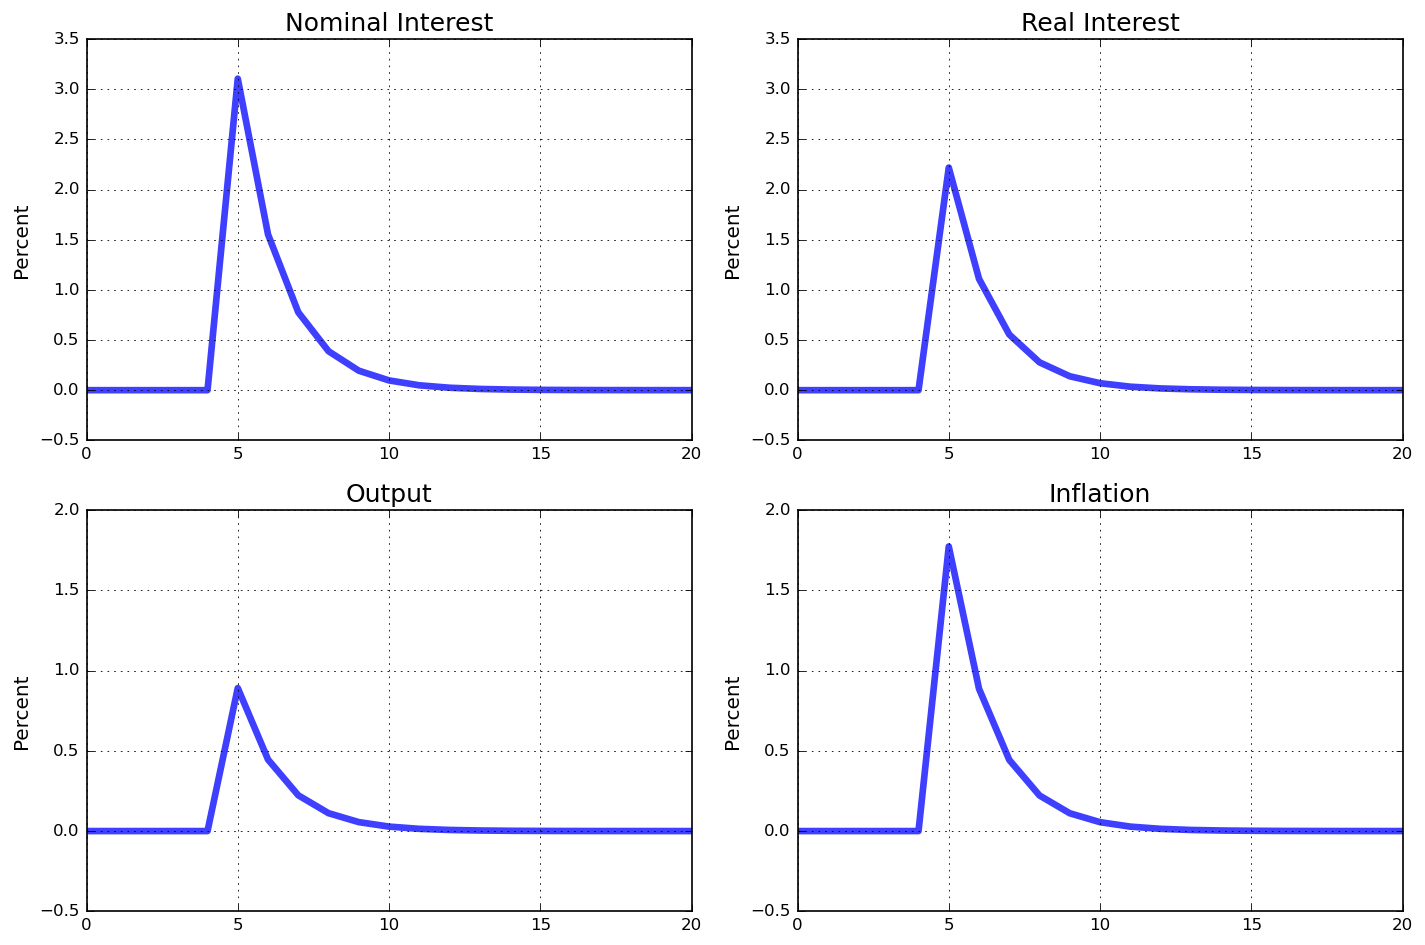
\includegraphics[height = 9cm]{fig_015_intro_nk_modeling_demand_shock.png}\end{center}
\end{figure}

%In order to produce Figure \ref{eqn:009a_Fig_Demand_Shock}, a simulation for $g_t$ has to be obtained first. To this, suppose that the demand shock is initially equal to zero:
%	\EE g_0 = 0
%	\FF
%that in period 1, there is a one unit shock to $g_t$:
%	\EE
%	\epsilon^g_1 & = & 1,
%	\FF
%and that there are no subsequent shocks to $g_t$:
%	\EE
%	\epsilon^g_2=\epsilon^g_3 = \cdots = 0
%	\FF
%With these assumptions and our calibrated value $\rho_g = 0.5$, we can compute:
%	\EE
%	g_1 = \rho_g g_0 +\epsilon^g_1 & = & 0.5 \times 0 + 1 = 1 \\
%	g_2 = \rho_g g_1 +\epsilon^g_2 & = & 0.5 \times 1 + 0 = 0.5 \\
%	g_3 = \rho_g g_2 +\epsilon^g_3 & = & 0.5 \times 0.5 + 0 = 0.25 \\
%	g_4 = \rho_g g_3 +\epsilon^g_4 & = & 0.5 \times 0.25 + 0 = 0.125 \\
%	& \vdots & \nonumber \\
%	g_T = \rho_g g_{T-1} +\epsilon^g_T & = & 0.5^{T-1} 
%	\FF
%Armed with computed values for $g_t$, output and inflation can be computed using the solution equations from above. Then the nominal interest rate can be computed using the monetary policy rule.

Returning to Figure \ref{fig_015_intro_nk_modeling_demand_shock}, we see that a 1 percent increase in the demand for goods increases total output by about 1.2 percent and raises inflation by about 1 percent. The central bank has responded to the higher output and inflation by raising the nominal interest rate by a little more than 2 percent while the real interest rate increases only by about 1.6 percent. As the demand shock dissipates, output, inflation, and the nominal interest rate decline back towards their steady state values.

The broad conclusion here is that a temporary demand shock will lead to a temporary business cycle expansion. The business cycle expansion is associated with an increase in the inflation rate. This leads us to conclude that demand-driven business cycle fluctuations are associated with procyclical inflation.



\subsection{Temporary Supply Shock}

Now, we will consider the effect of a persistent shock to the inflation rate. Again, we could compute the solution numerically or  by hand. To solve by hand, we assume that the inflation shock is the only shock in the model and write the equilibrium equations as:
	\EE
	y_t & = & E_t y_{t+1}  - \left( r_{t+1} - \bar{r}\right)\\
	\pi_t -\pi^T & = & \beta \left( E_t\pi_{t+1} - \pi^T\right)  + \kappa (y_t -\bar{y}) + u_t\\
	i_{t+1} & = & r_{t+1} + E_t \pi_{t+1}\\
	i_{t+1} & = & \bar{r} + \pi^T + \phi_{\pi}\left(\pi_t - \pi^T\right) + \phi_y \left(y_t - \bar{y}\right)
	\FF
Use the Fisher equation and the monetary policy rule to eliminate the nominal interest rate and the real interest rate from the model:
	\EE
	y_t & = & E_t y_{t+1} + E_t\pi_{t+1}  - \phi_{\pi}\left(\pi_t - \pi^T\right) - \phi_y \left(y_t - \bar{y}\right)\\
	\pi_t & = & (1-\beta) \pi^T + \beta \left( E_t\pi_{t+1} - \pi^*\right)  + \kappa (y_t -\bar{y}) + u_t
	\FF
This is another forward-looking system in two endogenous variables and one exogenous variables that can be solved with the method of undetermined coefficients. The solution to the system is:
	\EE
	y_t & = &\bar{y} -  \frac{\phi_{\pi}- \rho_u}{(1-\beta \rho_u)(1-\rho_u+\phi_y) + \kappa (\phi_{\pi} - \rho_u)}u_t \label{y_solve_u}
	\FF
and:
	\EE
	\pi_t & = & \pi^T + \frac{1-\rho_u}{(1-\beta \rho_u)(1-\rho_u+\phi_y) + \kappa (\phi_{\pi} - \rho_u)}u_t.\label{pi_solve_u}
	\FF
See Appendix \ref{sec:solution_supply} for the derivations. Together equations (\ref{y_solve_u}) and (\ref{pi_solve_u}) specify output and inflation as functions of the exogenous demand shock and fundamental model parameters.

The solution equations have a similar form to the solutions found under demand shocks. But there are clear differences. First, note that output is \emph{decreasing} with respect to the inflation shock $u_t$ while inflation is \emph{increasing} with respect to the shock. Hence, shocks to inflation send output and inflation in the opposite directions. Second, notice that as the central bank increases the degree to which it responds to changes in inflation $\phi_{\pi}$, inflation approaches its target but output does not. For example, taking $\phi_{\pi}\rightarrow\infty$, find:
	\EE
	y_t   & = &\bar{y} - \frac{1}{\kappa} u_t\\
	\pi_t & = & \pi^T.
	\FF
From this we infer that the central bank faces a trade-off when responding to shocks to inflation: each attempt to reduce the effect of the shock on inflation will induce a further reduction in output below the natural rate.


\begin{figure}[h] \caption{\label{fig_015_intro_nk_modeling_inflation_shock} \textbf{Inflation shock.} Impulse responses of the exogenous component of inflation, the nominal interest rate, output, and inflation to a 0.25 percent shock to the exogenous component of inflation. Inflation and interest rates are annualized.}
\begin{center}\hspace*{-.5cm}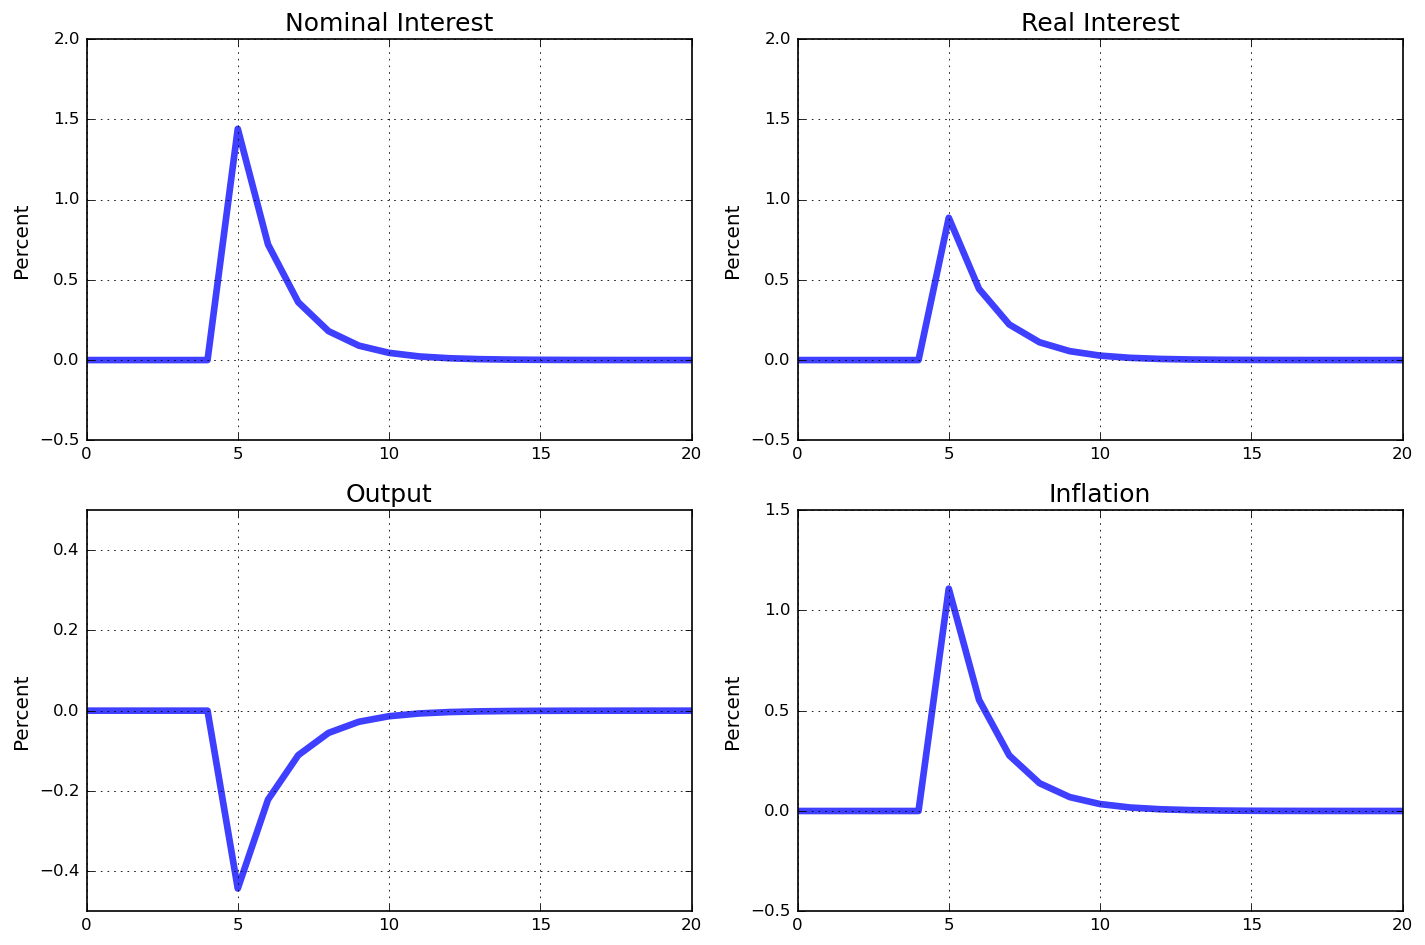
\includegraphics[height = 9cm]{fig_015_intro_nk_modeling_inflation_shock.png}\end{center}
\end{figure}

Figure \ref{fig_015_intro_nk_modeling_inflation_shock} plots impulse responses for $i_t$, $r_t$, $y_t$, and $\pi_t$ to a 0.25 percent exogenous increase in inflation.  The shock to inflation \emph{reduces} total output by about 0.6 percent below the natural rate and \emph{increases} inflation by about 1.5 percent. The central bank responds to the higher inflation by raising the nominal interest rate by a little less than 2 percent, also driving up the real interest rate by about 1.2 percent. As the supply shock dissipates, output, inflation, and the nominal interest rate return to their steady state values.

Now the broad conclusion here is that a temporary and positive inflation shock will lead to a temporary business cycle recession. The business cycle recession is associated with a higher inflation. This leads us to conclude that supply-driven business cycle fluctuations are associated with countercyclical inflation.


\subsection{Temporary Shock to Monetary Policy}

Finally, we will consider the effect of a persistent shock to the monetary policy rule. so now we solve the model assuming that the monetary policy shock is the only shock in the model. So write the equilibrium equations as:
	\EE
	y_t & = & E_t y_{t+1}  - \left( r_{t+1} - \bar{r}\right)\\
	\pi_t -\pi^T & = & \beta \left( E_t\pi_{t+1} - \pi^T\right)  + \kappa (y_t -\bar{y})\\
	i_{t+1} & = & r_{t+1} + E_t \pi_{t+1}\\
	i_{t+1} & = & \bar{r} + \pi^T + \phi_{\pi}\big(\pi_t - \pi^T\big) + v_t
	\FF
Now, use the Fisher equation and the monetary policy rule to eliminate the nominal interest rate and the real interest rate from the model:
	\EE
	y_t & = & E_t y_{t+1} + E_t\pi_{t+1}  - (1-\phi_{\pi})\pi^T - \phi_{\pi}\pi_t -  v_t\\
	\pi_t & = & (1-\beta) \pi^T + \beta \left( E_t\pi_{t+1} - \pi^*\right)  + \kappa (y_t -\bar{y})
	\FF
Again, this is a forward-looking system in two endogenous variables and one exogenous variable that can be solved with the method of undetermined coefficients. The solution to the system is:
	\EE
	y_t & = &\bar{y} - \frac{1-\beta\rho_v}{(1-\beta \rho_v)(1-\rho_v) + \kappa (\phi_{\pi} - \rho_v)}v_t \label{y_solve_v}
	\FF
and:
	\EE
	\pi_t & = & \pi^T - \frac{\kappa}{(1-\beta \rho_v)(1-\rho_v) + \kappa (\phi_{\pi} - \rho_v)} v_t.\label{pi_solve_v}
	\FF
Together equations (\ref{y_solve_v}) and (\ref{pi_solve_v}) specify output and inflation as functions of the exogenous monetary policy shock and fundamental model parameters. These equations are very similar to solution equations (\ref{y_solve_g}) and (\ref{pi_solve_g}) for output and inflation under the demand shock. This should not be surprising.

Figure \ref{fig_015_intro_nk_modeling_monetary_shock} plots impulse responses for $y_t$, $\pi_t$, and $i_t$ after a one-time one unit increase in $v_t$. Before analyzing the results, let's consider how the figure was constructed. The monetary policy shock leads to about a 1.3 percent reduction in output below the natural rate and inflation falls by out 0.35 percent. The responses of output and inflation are qualitatively similar to the responses to the demand shock in that both output and inflation move in the same directions. However, the difference is that in this case, the nominal interest rate rises just over 1 percent while it falls in response to the shock to the IS curve.


\input{figure_015_intro_nk_modeling_monetary_shock.tex}

\section{Conclusion}

The basic new-Keynesian model is a concise model of the dynamic relationship between GDP, inflation, and interest rates. Like the RBC model, the new-Keynesian model is founded on microeconomic principles. The distinguishing feature of the new-Keynesian approach is the micro-founded new-Keynesian Phillips curve which arrises as a consequence of an explicit model of price stickiness. The new-Keynesian Phillips curve implies a short-run trade-off between output and inflation and therefore a role for monetary policy that is not present in the RBC model.


\cleardoublepage
\begin{appendix}

\section{The Euler Equation in a Two-Period Model}

\subsection{Households}

A \emph{representative household} lives for two periods. The household receives utility from consuming goods in each period. The \emph{lifetime utility} to the household from consuming $C_0$ in the first period and $C_1$ in the second is denoted by $U(C_0,C_1)$ and is written as:
	\EE
	U(C_0,C_1) & = & u(C_0) + \beta u(C_1),  \label{eqn:two_per_utility}
	\FF
where $u(\cdot)$ is the period utility function. We assume that $u(\cdot)$ is strictly increasing and concave. The constant $\beta<1$ reflects the degree to which the household \emph{discounts} utility received in the future relative to utility received in the current period. Figure \ref{fig:two_per_util} depicts a typical period utility function.

	\begin{figure}[h] \caption{\label{fig:two_per_util} Representation of household preferences.}
	\begin{center}

	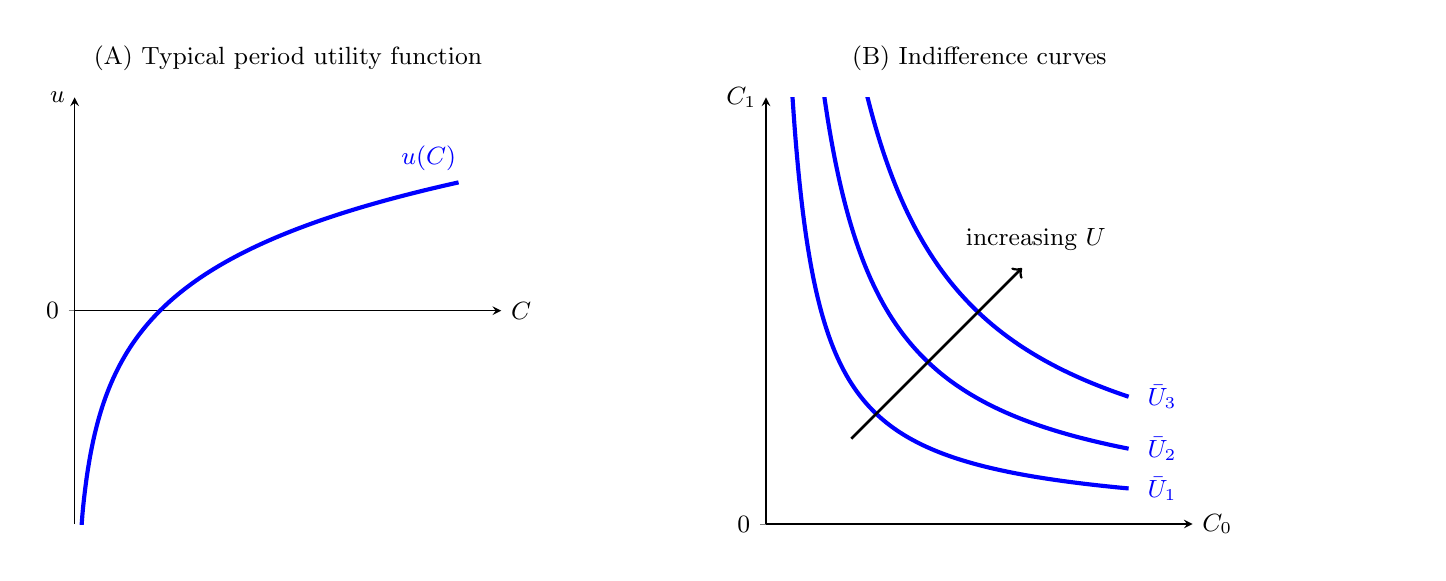
\begin{tikzpicture}
	\matrix{\begin{axis}[standard,%tiny,
    %scale only axis,
    font=\small,
    ytick={0},
    yticklabels={0},
    xtick={0},
    xticklabels={0},
    minor tick num=0,
    axis y line=left,
    axis x line=middle,
    xmin = 0,
    xmax = 5,
    ymin = -2.5,
    ymax = 2.5,
    xlabel style={at=(current axis.right of origin), anchor=west,text width=2.5 cm},
    ylabel style={left},
    xlabel=$C$,ylabel=$u$,
    title={(A) Typical period utility function}
	]
	\addplot[smooth,blue,mark=none,line width = 1.5pt,
	domain=0:4.5,samples=100]
	{ln(x)} node [pos=0.95,inner sep=2pt,label=above:$u(C)$] {};
	%\addplot[smooth,blue,mark=none,line width = 1.5pt,
	%domain=1:4,samples=100]
	%{exp(ln(2)+ln(2.5)-ln(x))} node [pos=0.95,inner sep=2pt,label=right:$\bar{U}^*$] {};
	%\addplot[blue,dotted,mark=,line width = 1pt]
	%coordinates{(0,3) (3,3) (3,0)};
	%\addplot[blue,solid,mark=*,line width = 1pt]
	%coordinates{(3,3)} node[pos=0.5, above, font=\footnotesize, yshift=0pt,xshift = 25pt] {endowment};
	%\addplot[magenta,dotted,mark=,line width = 1pt]
	%coordinates{(2,0) (2,2.5) (0,2.5)};
	%\addplot[magenta,solid,mark=*,line width = 1pt]
	%coordinates{(2,2.5)} ;
	\end{axis}
	&
	\begin{axis}[standard,%tiny,
    %scale only axis,
    font=\small,
    ytick={0},
    yticklabels={0},
    xtick={0},
    xticklabels={0},
    minor tick num=0,
    axis y line=left,
    axis x line=middle,
    xmin = 0,
    xmax = 5,
    ymin = 0,
    ymax = 5,
    xlabel style={at=(current axis.right of origin), anchor=west,text width=2.5 cm},
    ylabel style={left},
    xlabel=$C_0$,ylabel=$C_1$,
    title={(B) Indifference curves}
	]
	%\addplot[smooth,blue,mark=none,line width = 1.5pt,
	%domain=0:4.25,samples=100]
	%{exp(0.25-0.95*ln(x))} node [pos=1,inner sep=2pt,label=right:$\bar{u}_0$] {};
	\addplot[smooth,blue,mark=none,line width = 1.5pt,
	domain=0:4.25,samples=100]
	{exp(.5-0.95*ln(x))} node [pos=1,inner sep=2pt,label=right:$\bar{U}_1$] {};
	\addplot[smooth,blue,mark=none,line width = 1.5pt,
	domain=0:4.25,samples=100]
	{exp(1.25-0.95*ln(x))} node [pos=1,inner sep=2pt,label=right:$\bar{U}_2$] {};
	\addplot[smooth,blue,mark=none,line width = 1.5pt,
	domain=0:4.25,samples=100]
	{exp(1.775-0.95*ln(x))} node [pos=1,inner sep=2pt,label=right:$\bar{U}_3$] {};
	%\addplot[smooth,blue,mark=none,line width = 1.5pt,
	%domain=0:4.25,samples=100]
	%{exp(-0.95*ln(x))} node [pos=1,inner sep=2pt,label=right:$\bar{u}_0$] {};
	
	%\addplot[smooth,blue,mark=none,line width = 1.5pt,
	%domain=1:4,samples=100]
	%{exp(ln(2)+ln(2.5)-ln(x))} node [pos=0.95,inner sep=2pt,label=right:$\bar{U}^*$] {};
	%\addplot[blue,dotted,mark=,line width = 1pt]
	%coordinates{(0,3) (3,3) (3,0)};
	%\addplot[blue,solid,mark=*,line width = 1pt]
	%coordinates{(3,3)} node[pos=0.5, above, font=\footnotesize, yshift=0pt,xshift = 25pt] {endowment};
	%\addplot[magenta,dotted,mark=,line width = 1pt]
	%coordinates{(2,0) (2,2.5) (0,2.5)};
	%\addplot[magenta,solid,mark=*,line width = 1pt]
	%coordinates{(2,2.5)} ;
	\addplot[->,black,mark=none,line width = 1pt]
	coordinates{(1,1) (3,3)} node [pos=1,inner sep=2pt,xshift=5pt,label=above:increasing $U$] {};
	\end{axis}
	\\};
	\end{tikzpicture}
	\end{center}
	\end{figure}

The household has no initial wealth but receives income in each period that can be used to purchase consumption goods. In period 0, the household receives income $Y_0$ which it allocates between consumption in period 0 and saving for use in period 1. This implies a budget constraint for period 0:
	\EE
	C_0 & = & Y_0 - S_1,  \label{eqn:two_per_bc0}
	\FF
where $S_1$ represents savings for period 1. Saving is not required to be positive. If $S_1$ is less than zero, then we say that the household is borrowing against future its income. For every unit of income that the household saves in period 0, it receives $1+r_0$ units of income in period 1.\footnote{Likewise, for every unit of income borrowed against future income, the household must pay $1+r_0$ units in period 1.} We call $r_0$ the \emph{real interest rate} because it reflects the rate at which the household can transfer real goods -- as opposed to dollar-denominated quantities -- across time. Note that while $S_1$ has a subscript ``1'',  this quantity is in fact determined in period 0. 

In period 1, the household consumes its income $Y_1$ and its income from saving $(1+r_0)S_1$ which implies a budget constraint for the second period:
	\EE
	C_1 & = & Y_1 + (1+r_0)S_1.  \label{eqn:two_per_bc1}
	\FF
In writing this constraint, we are implicitly assuming that the household does not save in period 1. In principle there is no reason why this wouldn't be permissible, but since the household knows with certainty that there is no period 2, it is clear that saving in the last period would not be optimal.

The household's objective is to choose consumption in each period and a level of saving to maximize its lifetime utility (\ref{eqn:two_per_utility}) subject to the two budget constraints (\ref{eqn:two_per_bc0}) and (\ref{eqn:two_per_bc1}). We can express the optimization problem concisely as:
	\EE
	&&\max_{C_0,C_1,S_1} \; u(C_0) + \beta u(C_1)\\
	&& \; \; \; \;  \; \; \; \; \tn{s.t.} \; \; \; \; C_0 = Y_0 - S_1\\
	&&\; \; \; \; \; \; \; \; \; \; \; \; \; \; \; \; \; C_1 = Y_1 + (1+r_0)S_1.
	\FF
To solve this constrained optimization problem, we will use constraints to eliminate $C_0$ and $C_1$ from the problem so that we are left with an unconstrained optimization problem.\footnote{Alternatively, we could certainly use the method of Lagrange multipliers.} After making the substitutions, we obtain the simplified representation of the problem:
	\EE
	\max_{S_1} \; u( Y_0 - S_1) + \beta u\left[ Y_1 + (1+r_0)S_1\right]
	\FF
Next we solve the problem by setting derivative of the objective function with with respect to $S_1$ equal to zero:
	\EE
	-u'( Y_0 - S_1) + (1+r_0) \beta u'\left[ Y_1 + (1+r_0)S_1\right] & = & 0 \label{eqn:two_per_s1_foc},
	\FF
where $u'(\cdot)$ denotes the period marginal utility of consumption. Equation (\ref{eqn:two_per_s1_foc}) is the \emph{first-order condition} for the optimal choice of $S_1$. Notice that the arguments of $u'(\cdot)$ in equation (\ref{eqn:two_per_s1_foc}) are still $C_0$ and $C_1$. This means that we can rewrite the first-order condition for $S_1$ in terms of consumption:
	\EE
	\boxed{u'(C_0) = \beta (1+ r_0) u'(C_1)} \label{two_per_euler}
	\FF
Equation (\ref{two_per_euler}) is called the household's \emph{consumption Euler equation}. The consumption Euler equation -- or just Euler equation, for short -- indicates that the optimal choice of consumption in period 0 depends on consumption in period 1 and, of course, the interest rate which represents the price of period 0 goods in terms of period 1 goods. Equation (\ref{two_per_euler}) does not directly link household consumption with income, but it does provide us with a way to compute consumption in each period given a real interest rate and values for household income in each period.

We will assume that the period utility function is the natural logarithm of consumption:
	\EE
	u(C) & = & \log C.
	\FF
With this utility function, the household's Euler equation is expressed as:
	\EE
	\boxed{\frac{1}{C_0} = \frac{\beta (1+ r_0)}{C_1}} \label{two_per_euler}
	\FF


	\begin{figure}[t] \caption{\label{fig:two_per_opt_saving} Saving and borrowing behavior is determined by the relative sizes of income in each period.}
	\begin{center}

	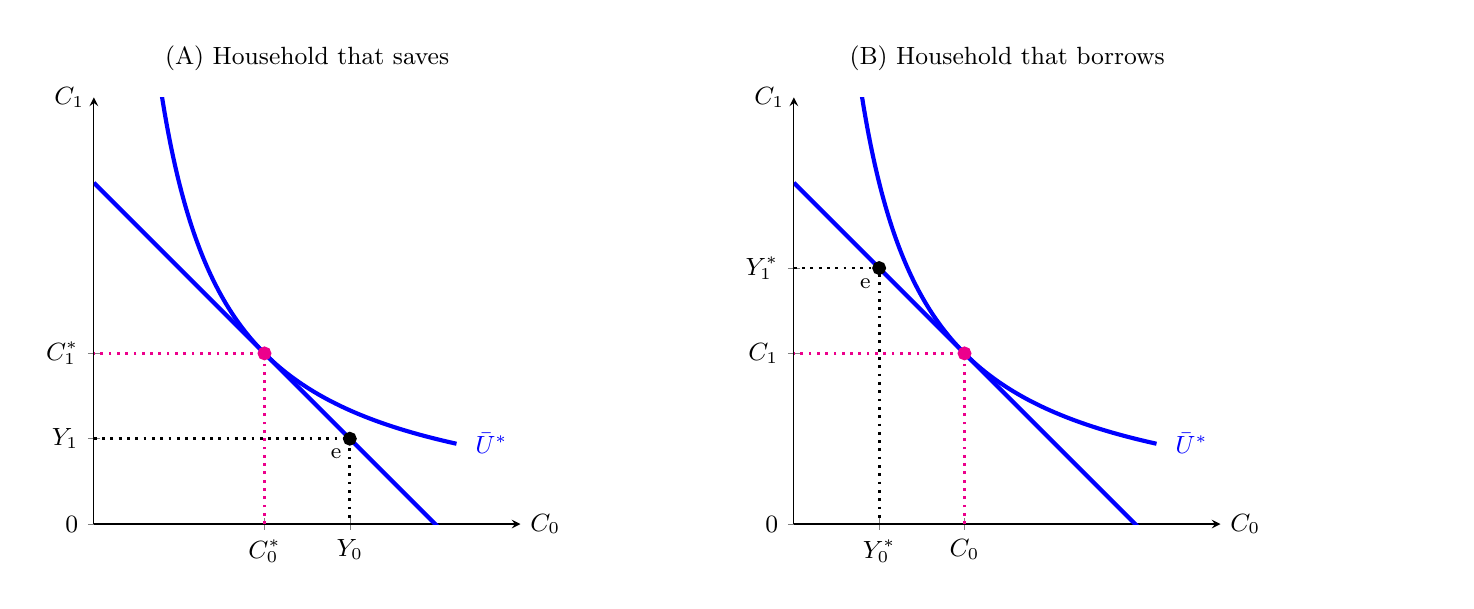
\begin{tikzpicture}
	\matrix{\begin{axis}[standard,%tiny,
    %scale only axis,
    font=\small,
    ytick={0,1,2},
    yticklabels={0,$Y_1$,$C_1^*$},
    xtick={0,2,3},
    xticklabels={0,$C_0^*$,$Y_0$},
    minor tick num=0,
    axis y line=left,
    axis x line=middle,
    xmin = 0,
    xmax = 5,
    ymin = 0,
    ymax = 5,
    xlabel style={at=(current axis.right of origin), anchor=west,text width=2.5 cm},
    ylabel style={left},
    xlabel=$C_0$,ylabel=$C_1$,
    title={(A) Household that saves}
	]
	\addplot[smooth,blue,mark=none,line width = 1.5pt,
	domain=0:4.25,samples=100]
	{4-x} node [pos=1,inner sep=2pt,label=right:$\bar{u}_0$] {};
	\addplot[smooth,blue,mark=none,line width = 1.5pt,
	domain=0:4.25,samples=100]
	{exp(ln(2) + ln(2) - ln(x))} node [pos=1,inner sep=2pt,label=right:$\bar{U}^*$] {};
	\addplot[black,dotted,mark=,line width = 1pt]
	coordinates{(0,1) (3,1) (3,0)};
	\addplot[black,solid,mark=*,line width = 1pt]
	coordinates{(3,1)} node[pos=0.5, below, font=\footnotesize, yshift=0pt,xshift = -5pt] {e};
	\addplot[magenta,dotted,mark=,line width = 1pt]
	coordinates{(2,0) (2,2) (0,2)};
	\addplot[magenta,solid,mark=*,line width = 1pt]
	coordinates{(2,2)} ;
	\end{axis}
	&
	\begin{axis}[standard,%tiny,
    %scale only axis,
    font=\small,
    ytick={0,2,3},
    yticklabels={0,$C_1$,$Y_1^*$},
    xtick={0,1,2},
    xticklabels={0,$Y_0^*$,$C_0$},
    minor tick num=0,
    axis y line=left,
    axis x line=middle,
    xmin = 0,
    xmax = 5,
    ymin = 0,
    ymax = 5,
    xlabel style={at=(current axis.right of origin), anchor=west,text width=2.5 cm},
    ylabel style={left},
    xlabel=$C_0$,ylabel=$C_1$,
    title={(B) Household that borrows}
	]
	\addplot[smooth,blue,mark=none,line width = 1.5pt,
	domain=0:4.25,samples=100]
	{4-x} node [pos=1,inner sep=2pt,label=right:$\bar{u}_0$] {};
	\addplot[smooth,blue,mark=none,line width = 1.5pt,
	domain=0:4.25,samples=100]
	{exp(ln(2) + ln(2) - ln(x))} node [pos=1,inner sep=2pt,label=right:$\bar{U}^*$] {};
	\addplot[black,dotted,mark=,line width = 1pt]
	coordinates{(0,3) (1,3) (1,0)};
	\addplot[black,solid,mark=*,line width = 1pt]
	coordinates{(1,3)} node[pos=0.5, below, font=\footnotesize, yshift=0pt,xshift = -5pt] {e};
	\addplot[magenta,dotted,mark=,line width = 1pt]
	coordinates{(2,0) (2,2) (0,2)};
	\addplot[magenta,solid,mark=*,line width = 1pt]
	coordinates{(2,2)} ;
	\end{axis}
	\\};
	\end{tikzpicture}
	\end{center}
	\end{figure}

%\input{figure_015_intro_nk_modeling_saving_borrowing}

\section{Derivation of the Dynamic IS Relationship}

In the two-period model without uncertainty, we found that an Euler equation for a representative household 
	\EE
	\frac{1}{C_0} & = & \beta \frac{1}{C_1} (1+r_{0})
	\FF
Supposing there there is no investment, government purchases, or net exports, then $Y = C$ in every period:
	\EE
	\frac{1}{Y_0} & = & \beta \frac{1}{Y_1} (1+r_{0})
	\FF
Next, take the log of each side to obtain a linear representation of the Euler equation:
	\EE
	\log Y_0 & = & \log \beta - \log Y_1 + \log \left(1+r_{0}\right)
	\FF
Rearranging and defining $\bar{r} \equiv -\log \beta$ as the natural rate of interest, obtain:
	\EE
	y_0 & = & y_1 - (r_{0}-\bar{r}).
	\FF
We have now obtained an expression based on the household's Euler equation that links (log) output today with (log) output in one period and the difference between the actual real interest rate and the natural rate of interest.

So far, we have assumed no uncertainty; $y_1$ is known in advance. In reality, future income is not known in advance because future income is subject to the realization of unpredictable macroeconomic shocks. I incorporate uncertainty into the model by replacing $y_1$ with its expectation conditional on period 0 information $E_0y_1$. I also append a demand shock to the end off the equation:
	\EE
	y_0 & = & E_0y_1 -(r_{0}-\bar{r}) + g_0
	\FF
Next, we simply note that the previous expression will hold for any two adjacent time periods $t$ and $t+1$ and obtain:
	\EE
	\boxed{y_t = E_ty_{t+1} -(r_{t} -\bar{r}) + g_t}
	\FF
	
\section{Derivation of the Dynamic AS Relationship}
	
\subsection{Problem Setup}

Consider a model in which a large number of monopolistically competitive firms produce output in two adjacent time periods. As monopolistic competitors, each firm has the ability to set the price of its product. Suppose that, absent other considerations, each firm would like to set the price of its product in each period according to the following rule:
	\EE
	p^*_t & = & p_t + \eta( y_t-\bar{y}) + \tilde{u}_t,
	\FF
where $p^*_t$ is the log of each firm's ideal price, $p_t$ is the log of the aggregate price level and $y_t$ is the log of output. $\tilde{u_t}$ is a random shock to the cost of producing goods and can be associated with events like shocks to the prices of oil or food. The constant $\eta\geqslant 0$ reflects the degree of market power held by the typical firm. If firms were competitive price takers, then $\eta = 0$.

In each period, a typical firm $j$ incurs two costs related to price-setting. First, the firm incurs a cost that is increasing with respect to the squared difference between the firms actually price and its ideal price. Second, the firm incurs a cost for changing its price at a rate that is different from average inflation $\pi^*$. Together, the costs incurred in period $t$ associated with price-setting are:
	\EE
	\left( p_t^j - p^*_t\right)^2 + \phi \left(p^j_t - p^j_{t-1}-\pi^*\right)^2.
	\FF
It is apparent that in the model the firm faces a trade-off between setting the price of its product equal to its ideal price and simply adjusting its price to keep up with average inflation. This tradeoff is what will give rise to the upward-sloping supply curve.
	
\subsection{Optimization}

The firm chooses $p^j_0$ to minimize its costs:
	\EE
	\min_{p_0^j} \left( p_0^j - p^*_0\right)^2 + \phi \left(p_0^j - p_{-1}^j\right)^2 + \beta E_0\left[\left( p_1^j - p^*_1\right)^2 + \phi \left(p_1^j - p_{0}^j\right)^2\right].
	\FF
The first-order optimality condition for $p_0^j$ is given by:
	\EE
	p_0^j - p^*_0 + \phi \left(p_0^j - p_{-1}^j\right) - \phi \beta E_1\left(p_1^j - p_{0}^j\right) = 0
	\FF
Recall that:
	\EE
	p_0^j - p_0 - \eta ( y_0-\bar{y}) - \tilde{u}_0 + \phi \left(p_0^j - p_{-1}^j\right) - \phi \beta E_0\left(p_1^j - p_{0}^j\right) = 0
	\FF
And since every firm solves the same problem, $p_t^j = p_t^i$ for any firms $i$ and $j$. Therefore:
	\EE
	\phi\left(p_0 - p_{-1}\right)  & = & \phi \beta E_0\left(p_1 - p_{0}\right) + \eta (y_0-\bar{y}) + \tilde{u}_0\\
	p_0 - p_{-1}  & = & \beta E_0\left(p_1 - p_{0}\right) + \frac{\eta}{\phi} (y_0-\bar{y}) + \frac{1}{\phi}\tilde{u}_0
	\FF
Finally, we make use of the fact that $\pi_t = p_t - p_{t-1}$ and obtain:
	\EE
	\pi_0 & = & \beta E_0\pi_1 + \kappa (y_0-\bar{y})  + u_0
	\FF
where:
	\EE
	\kappa \equiv \frac{\eta}{\phi}
	\FF
and:
	\EE
	u_{0} & = & \frac{1}{\phi}\tilde{u}_0
	\FF
	
\subsection{Extension to Infinite-Horizon}

The analysis presented here focused on a two-period model, but we could extend the model to an infinite horizon model. In so doing, we would find that the inflation relationship uncovered above would hold for any two adjacent periods $t$ and $t+1$:
	\EE
	\boxed{\pi_t = \beta E_t\pi_{t+1} + \kappa (y_t - \bar{y}) + u_t}
	\FF
And this is the dynamic AS relationship.

\section{Model Solution}

\subsection{Demand Shock}
\label{sec:solution_demand}

After eliminating the real and nominal interest rates from the model, there are two equations that describe output and inflation given the demand shock:
	\EE
	y_t & = & E_t y_{t+1} + E_t\pi_{t+1}  - (1-\phi_{\pi})\pi^T - \phi_{\pi}\pi_t - \phi_y y_t + \phi_y \bar{y} +  g_t\\
	\pi_t & = & (1-\beta) \pi^T + \beta \left( E_t\pi_{t+1} - \pi^T\right)  + \kappa (y_t -\bar{y})
	\FF
We will solve this using the method of undetermined coefficients.

\subsubsection{Guess}

Guess that the solution has the following form:
	\EE
	y_t & = & \bar{y} + a g_t\\
	\pi_t & = & \pi^T + b g_t
	\FF
This is a good guess because we know that in the steady state $g_t = 0$, $y_t = \bar{y}$, and $\pi_t = \pi^T$. Now, the guess implies:
	\EE
	E_ty_{t+1} & = & \bar{y} + a \rho_gg_t\\
	E_t\pi_{t+1} & = & \pi^T + b \rho_gg_t
	\FF
Now we can solve for $a$ and $b$.	


\subsubsection{Solve}

Start with the first equation of the system and use the guess to eliminate $E_t\pi_{t+1}$, $E_ty_{t+1}$, and $\pi_t$ from the right-hand side of the equation:
	\EE
	y_t & = & E_t y_{t+1} + E_t\pi_{t+1}  - (1-\phi_{\pi})\pi^T - \phi_{\pi}\pi_t - \phi_y y_t + \phi_y \bar{y} +  g_t\\
	(1+\phi_y ) y_t & = & (1+\phi_y ) \bar{y} + a \rho_gg_t + \pi^T + b \rho_gg_t - (1-\phi_{\pi})\pi^T - \phi_{\pi}( \pi^T + b g_t) + g_t\\
	& = & (1+\phi_y )\bar{y} + a \rho_gg_t + b \rho_gg_t - \phi_{\pi}b g_t + g_t\\
	y_t & = & \bar{y} + \frac{1}{1+\phi_y }\left[a \rho_g + b (\rho_g - \phi_{\pi}) + 1\right]g_t
	\FF
Therefore:
	\EE
	\boxed{a  =  \frac{1}{1+\phi_y }\left[a \rho_g + b (\rho_g - \phi_{\pi}) + 1\right]}
	\FF
Next, use the dynamic AS equation to write:
	\EE
	\pi_t & = & (1-\beta) \pi^T + \beta \left( \pi^T + b \rho_gg_t - \pi^T\right)  + \kappa (\bar{y} + a g_t -\bar{y})\\
	& = & \pi^T + \beta b \rho_gg_t + \kappa a g_t\\
	& = & \pi^T + \left[ \beta b \rho_g + \kappa a \right]g_t
	\FF
Therefore:
	\EE
	\boxed{b = \beta b \rho_g + \kappa a}
	\FF
Now, take the two boxed equations and solve for $a$ and $b$:
	\EE
	\boxed{a = \frac{1-\beta\rho_g}{(1-\beta\rho_g)(1-\rho_g+\phi_y)+ \kappa(\phi_{\pi}-\rho_g)} }
	\FF
	and:
	\EE
	\boxed{b = \frac{\kappa}{(1-\beta\rho_g)(1-\rho_g+\phi_y)+ \kappa(\phi_{\pi}-\rho_g)}}
	\FF
You should \emph{verify} that these equations are in fact solutions to the original system.

\subsection{Monetary Policy Shock}
\label{sec:solution_monetary_policy}

After eliminating the real and nominal interest rates from the model, there are two equations that describe output and inflation given the monetary policy shock:
	\EE
	y_t & = & E_t y_{t+1} + E_t\pi_{t+1}  - (1-\phi_{\pi})\pi^T - \phi_{\pi}\pi_t - \phi_y y_t + \phi_y \bar{y} - v_t\\
	\pi_t & = & (1-\beta) \pi^T + \beta \left( E_t\pi_{t+1} - \pi^T\right)  + \kappa (y_t -\bar{y})
	\FF
Apparently, the monetary policy shock enters the reduced model in the same way that the demand shock does but with the opposite sign. Therefore, the solution has the following form:
	\EE
	y_t & = & \bar{y} + a v_t\\
	\pi_t & = & \pi^T + b v_t,
	\FF
with: 
	\EE
	\boxed{a = -\frac{1-\beta\rho_v}{(1-\beta\rho_v)(1-\rho_v+\phi_y)+ \kappa(\phi_{\pi}-\rho_v)} }
	\FF
	and:
	\EE
	\boxed{b = -\frac{\kappa}{(1-\beta\rho_v)(1-\rho_v+\phi_y)+ \kappa(\phi_{\pi}-\rho_v)}}
	\FF
You should \emph{verify} that these equations are in fact solutions to the original system.

\subsection{Supply Shock}
\label{sec:solution_supply}

After eliminating the real and nominal interest rates from the model, there are two equations that describe output and inflation given the inflation shock:
	\EE
	y_t & = & E_t y_{t+1} + E_t\pi_{t+1}  - (1-\phi_{\pi})\pi^T - \phi_{\pi}\pi_t - \phi_y y_t + \phi_y \bar{y} \\
	\pi_t & = & (1-\beta) \pi^T + \beta \left( E_t\pi_{t+1} - \pi^T\right)  + \kappa (y_t -\bar{y}) + u_t
	\FF
We will solve this using the method of undetermined coefficients.

\subsubsection{Guess}

Guess that the solution has the following form:
	\EE
	y_t & = & \bar{y} + a u_t\\
	\pi_t & = & \pi^T + b u_t
	\FF
This is a good guess because we know that in the steady state $u_t = 0$, $y_t = \bar{y}$, and $\pi_t = \pi^T$. Now, the guess implies:
	\EE
	E_ty_{t+1} & = & \bar{y} + a \rho_uu_t\\
	E_t\pi_{t+1} & = & \pi^T + b \rho_uu_t
	\FF
Now we can solve for $a$ and $b$.	


\subsubsection{Solve}

Start with the first equation of the system and use the guess to eliminate $E_t\pi_{t+1}$, $E_ty_{t+1}$, and $\pi_t$ from the right-hand side of the equation:
	\EE
	y_t & = & E_t y_{t+1} + E_t\pi_{t+1}  - (1-\phi_{\pi})\pi^T - \phi_{\pi}\pi_t - \phi_y y_t + \phi_y \bar{y}\\
	(1+\phi_y) y_t & = & (1+\phi_y)\bar{y} + a \rho_uu_t + \pi^T + b \rho_uu_t - (1-\phi_{\pi})\pi^T - \phi_{\pi}( \pi^T + b u_t)\\
	& = & (1+\phi_y)\bar{y} + a \rho_uu_t + b \rho_uu_t - \phi_{\pi}b u_t \\
	y_t & = & \bar{y} + \frac{1}{1+\phi_y}\left[a \rho_u + b (\rho_u - \phi_{\pi})\right]u_t
	\FF
Therefore:
	\EE
	\boxed{a  = \frac{1}{1+\phi_y}\left[a \rho_u + b (\rho_u - \phi_{\pi})\right]}
	\FF
Next, use the dynamic AS equation to write:
	\EE
	\pi_t & = & (1-\beta) \pi^T + \beta \left( \pi^T + b \rho_gg_t - \pi^T\right)  + \kappa (\bar{y} + a g_t -\bar{y}) + u_t\\
	& = & \pi^T + \beta b \rho_uu_t + \kappa a u_t + u_t\\
	& = & \pi^T + \left[ \beta b \rho_u + \kappa a + 1\right]u_t
	\FF
Therefore:
	\EE
	\boxed{b = \beta b \rho_u + \kappa a + 1}
	\FF
Now, take the two boxed equations and solve for $a$ and $b$:
	\EE
	\boxed{a = -\frac{(\phi_{\pi} - \rho_u)}{(1-\beta\rho_u)(1-\rho_u+\phi_y)+ \kappa(\phi_{\pi}-\rho_u)}}
	\FF
	and:
	\EE
	\boxed{b = \frac{1-\rho_u+\phi_y}{(1-\beta\rho_u)(1-\rho_u+\phi_y)+ \kappa(\phi_{\pi}-\rho_u)}}
	\FF
You should \emph{verify} that these equations are in fact solutions to the original system.


\end{appendix}

%%%%%%%%%%%%%%%%%%%%%%%%%%%%%%%%%%%%%%%%%%%%%%%%%%%%%%%%%%%%%%%%%
%%%%%%%%%%%%%%%%%%%%%%%%%%%%%%%%%%%%%%%%%%%%%%%%%%%%%%%%%%%%%%%%%%%%
%\bibliography{EconRef}


\end{document}

%%%%%%%%%%%%%%%%%%%%%%%%%%%%%%%%%%
%%%%%%%%%%%%%%%%%%%%%%%%%%%%%%%%%%
%%% Example table %%%%%%%%%%%%%%%%
%%%%%%%%%%%%%%%%%%%%%%%%%%%%%%%%%%
%%%%%%%%%%%%%%%%%%%%%%%%%%%%%%%%%%


\begin{landscape}
\begin{table}[] \caption{\label{} Optimal monetary policy from Schmitt-Groh\'{e} and Uribe 2007}

\
\begin{tabular}{llllllll} \hline
 & $\alpha_{\pi}$ & $\alpha_y$ & $\alpha_R$ &  Conditional welfare & Unconditional welfare & $\sigma_{\pi}$ & $\sigma_{R}$ \\
 & & & & cost ($\lambda^c \times 100$) & cost ($\lambda^c \times 100$)\\ \hline
 \textbf{A. The cashless economy} {\rule[0mm]{0mm}{5mm}}\\
 Ramsey Policy & - & - & - & ~0 & 0 &0.01 &  0.27 \\
 Optimized Rules \\
 Contemporaneous ($i=0$)\\
 {\rule[0mm]{1.0mm}{0mm}} Smoothing & 3 & 0.01 & 0.84 & ~0.000 & 0.000 & 0.04 &  0.29 \\
 {\rule[0mm]{1.0mm}{0mm}} No Smoothing & 3 & 0.00 & - & ~0.000 & 0.001 & 0.14 &  0.42 \\
 Backward ($i=1$) & 3 & 0.03 & 1.71 & ~0.001 & 0.001 & 0.10 &  0.23 \\
 Forward ($i=-1$) & 3 & 0.07 & 1.58 & ~0.002 & 0.003 & 0.19 & 0.27 \\
 Nonoptimized rules\\
 Taylor rule ($i=0$) & 1.5 & 0.5 & - & ~0.451 & 0.522 & 3.19 & 3.08\\
 Simple Taylor rule & 1.5 & - & - & ~0.014 & 0.019 & 0.58 & 0.87\\
 \\
 \textbf{B. The monetary economy} {\rule[0mm]{0mm}{5mm}}\\
 Ramsey Policy & - & - & - & ~0 & 0 &0.01 & 0.27 \\
 Optimized Rules \\
 Contemporaneous ($i=0$)\\
 {\rule[0mm]{1.0mm}{0mm}} Smoothing & 3 & 0.01 & 0.80 & ~0.000 & 0.000 & 0.04 & 0.29 \\
 {\rule[0mm]{1.0mm}{0mm}} No Smoothing & 3 & 0.00 & - & ~0.001 & 0.001 & 0.14 & 0.41 \\
 Nonoptimized rules\\
 Taylor rule ($i=0$) & 1.5 & 0.5 & - & ~0.598 & 0.709 & 3.93 & 3.76\\
 {\rule[3mm]{0mm}{0mm}}Simple Taylor rule & 1.5 & - & - & ~0.011 & 0.015 & 0.56 & 0.85\\\hline
 \end{tabular}
\end{table}

\end{landscape}







%%%%%%%%%%%%%%%%%%%%%%%%%%%%%%%%%%
%%%%%%%%%%%%%%%%%%%%%%%%%%%%%%%%%%
%%% Example figure and graphic %%%
%%%%%%%%%%%%%%%%%%%%%%%%%%%%%%%%%%
%%%%%%%%%%%%%%%%%%%%%%%%%%%%%%%%%%


\begin{figure}[h] \caption{\label{} The welfare cost of responding to output: varying $\alpha_y$ holding $\alpha_{\pi} =3$ and $\alpha_R = 0$.}
\includegraphics[height = 10cm]{fig1.png}
\end{figure}

